% !TeX program = xelatex
\documentclass[10pt, landscape, oneside]{article}

%Import our packages, see import.tex
\usepackage{import}
\import{../}{imports}
\usepackage[margin=10pt, heightrounded,landscape]{geometry}
\usepackage{multicol}

%assignment configuration
\author{Me}
\title{Cribsheet}

% Set up page style
\pagestyle{empty}


%resize sectioning
\makeatletter
\renewcommand{\section}{\@startsection{section}{1}{0mm}%
                                {-1ex plus -.5ex minus -.2ex}%
                                {0.5ex plus .2ex}%x
                                {\normalfont\large\bfseries}}
\renewcommand{\subsection}{\@startsection{subsection}{2}{0mm}%
                                {-1explus -.5ex minus -.2ex}%
                                {0.5ex plus .2ex}%
                                {\normalfont\footnotesize\bfseries}}
\renewcommand{\subsubsection}{\@startsection{subsubsection}{3}{0mm}%
                                {-2ex plus -.5ex minus -.2ex}%
                                {-1ex plus .2ex}%
                                {\normalfont\footnotesize\bfseries}}
\makeatother

\providecommand{\qdef}[2]{{\textbf{#1}{ }} &{#2}} %hfill shortcut
\providecommand{\wdef}[4]{{\textbf{#1}{ }} {#2}, &{\textbf{#3}{ }} {#4}} %hfill shortcut

\providecommand{\pxf}{P_{\mathbf{X}}(f)}
\providecommand{\pyf}{P_{\mathbf{y}}(f)}
\providecommand{\hf}{\mathbf{H}(f)}
\providecommand{\xf}{\mathbf{X}(f)}
\providecommand{\yf}{\mathbf{Y}(f)}
\providecommand{\wt}{\operatorname{wt}} %Hamming weight


\usepackage[nodisplayskipstretch]{setspace}
\usepackage{caption}
\captionsetup{justification=justified,singlelinecheck=false,font=small}
\setstretch{1}
\begin{document}

% Spacing Adjustments.
% Updated to not destroy matrices
\setlength{\parindent}{0pt}
\setlength{\parskip}{2pt}
\setlength{\belowdisplayskip}{-0.5ex}
\setlength{\abovedisplayskip}{-0.5ex}
\setlength{\belowdisplayshortskip}{-0.5ex}
\setlength{\abovedisplayshortskip}{-0.5ex}
\setlist[itemize]{leftmargin=*,noitemsep}
\setlist[enumerate]{leftmargin=*,noitemsep}
\setlength{\partopsep}{0pt plus 1pt minus 0pt}
\raggedright


% Spacing Adjustments.
% Updated to not destroy matrices
\setlength{\parindent}{0pt}
\setlength{\parskip}{2pt}
\setlength{\belowdisplayskip}{-0.5ex}
\setlength{\abovedisplayskip}{-0.5ex}
\setlength{\belowdisplayshortskip}{-0.5ex}
\setlength{\abovedisplayshortskip}{-0.5ex}
\setlist[itemize]{leftmargin=*,noitemsep}
\setlist[enumerate]{leftmargin=*,noitemsep}
\setlength{\partopsep}{0pt plus 1pt minus 0pt}
\raggedright


% \maketitle  % Uncomment if necessary




% Template 1
% \begin{multicols}{4}
% \setlength{\premulticols}{4pt}
% \setlength{\postmulticols}{4pt}
% \setlength{\multicolsep}{4pt}
% \setlength{\columnsep}{10pt}
% %\small
% \footnotesize


\begin{multicols}{6}
\setlength{\premulticols}{1pt}
\setlength{\postmulticols}{1pt}
\setlength{\multicolsep}{1pt}
\setlength{\columnsep}{-2pt}
\tiny

\setlength{\columnseprule}{1pt}
\def\columnseprulecolor{\color{black}}
\providecommand{\problemdivider}{\textcolor{gray}{\rule{\columnwidth}{1pt}}}

\boxed{\textcolor{red}{\textbf{Updated \today\, at \,\currenttime\hfill}}}


\problem{A}
\subsection*{Store\&Frwd PcktSw Delay}

\begin{itemize}[noitemsep]
    \item $N$:No.Links, $P$: No.Packets
    \item $L$: DataLength, $R$: linkRate
    \item End-End Delay: $t_{end-to-end}=(N+P)(L/R)$
    \item Trans Delay: arrival of 1st and last Bit
    \item Prop Delay: transmis. of 1st and arrival of 1st Bit
\end{itemize}






\problem{B}
\subsection*{Signals}


\begin{itemize}[noitemsep]
    \item EnergyJ: $\norm{x}^2_2=\norm{\bf{x}}^2_2$ 
    \item Pwr.Spc.DstyW/Hz $P_{\mathbf{X}}$: $\lim\limits_{d\to\infty} |\mathbf{X}_d (f)|^2/d$ 
    \item Trunc. $\mathbf{X}_d (f)$: $\cal{F}\{x(t)\cdot\chi[-d/2,+d/2]\}$ 
    \item E.Spec.Dsty J/Hz: $|\mathbf{X}(f)|^2\in\real^\Omega$ 
    \item Pwr $P_x$(2defs): $ \lim\limits_{d\to\infty}d^{-1}\int|x(t)|^2\chi_d dt$ 
    \item Pwr $P_x$(densDef): $\int P_{\bf{X}}$ 
    \item Sine.Pwr $x=A\cos(2\pi f_c t + \theta)$: $P_x=A/2$ 
    \item Abs. Bandwidth: $\inf \{(b-a),\,\supp{x}\subseteq[a,b]\}$ 
    \item Center Frequency: ${(a+b)}/2$
\end{itemize}



\subsection*{DSBLC AM Modulation}
%DSB LC

\begin{itemize}[noitemsep]
     \item DSB-LC AM, $s_{LC}(t)$: $A_c[1+km(t)]\cos(2\pi f_c t)$ 
     \item LC f.Dom, $\bf{S}_{LC}(f)$: $(A_c/2)[\delta(f-f_c) + \delta(f+f_c)]\allowbreak {(A_c/2)}[\mathbf{M}(f-f_c) + \mathbf{M}(f+f_c)]$ 
     \item $k$: no phase reversal: $1+km(t)\geq0$ 
     \item AM ModIndex $\phi$: $\phi=-km_{min} \leq 1$ 
     \item \% Mod: $100\phi$ 
     \item Under/Over Mod: $\phi<1$ or $\phi > 1$ 
\end{itemize}


\subsection*{ISI/AWGN}
\begin{itemize}[noitemsep]
    \item Shannon AWGN: $\Epsilon_{max}=\log_2(1+SNR)$
    \item Nyquist ISI: $\Epsilon_{sym}=f_s/B\leq 1$
    \item Eff. Brate $R_b$: $f_s\log_2|\mathcal{A}|$
\end{itemize}

\subsection*{Parity}
\begin{itemize}[noitemsep]
    \item Data $\{d_i\}_{i^{k-1}}$: ParityCheckBit $d_k$
    \item EvenP Check: $d_k = \oplus_{i}^{k-1}d_i$
    \item EvenP Verify: $\oplus^{k}_i d_{i}=0$
    \item OddP Check: $d_k = \odot_{i}^{k-1}d_i$
    \item OddP Verify: $\odot^{k}_i d_{i}=0$
\end{itemize}

\subsection*{CRC}
\begin{itemize}[noitemsep]
    \item $D$ data, $k$ bits: deg=$k-1$
    \item $G$ genpoly: deg=$n-k$
    \item $R$ FCS,remainder: deg=$n-k-1$
    \item Detect OddErrors: incl. $x+1$
    \item Detect SinglErrors: incl. $2+$ terms
\end{itemize}
\tiny{Irreducible polynomial of degree $m$, not divisible by any polynomial with degree $0<k<m$.\\
        Primitive polynomial of degree $m$, not divisible by any polynomial in the form $x^k + 1$, $0<k<2^m$\\
        If $G$ is an irreducible polynomial of degree $L$, then CRC can detect all BURST errors of $0<k<L$.
        If $G$ is a primitive polynomial of degree $L$, then CRC can detect all two-bit errors separated by $N<2^L$ bits.}
\subsubsection*{CRC steps}

\begin{itemize}[noitemsep]
    \item Step1: find n, k
    \item Step2: shift $D$ by $n-k$ bits
    \item Step3: $R(X)$ by rmndr of $X^{n-k}D(X)/G(X)$
    \item Step4: Concat $T(X)=X^{n-k}D(X) + R(X)$
\end{itemize}
\subsubsection*{Internet Checksum}

\begin{itemize}[noitemsep]
    \item Given: HEX chunks $[x^i_1 x^i_2 x^i_3 x^i_4]_{i}$, add one more chunk
    \textbf{Step1}  sum all chunks in hex\\
    \textbf{Step2}  if overflow, use 1COF (\verb|2DCD7->DCD9|)\\
    \textbf{Step3}  take 1cCOMP, (\verb|DCD9->FFFF-DCD9=2326|)\\
    \textbf{Step4}  internetchecksum is \verb|2326|\\
    \textbf{Verify}  sum all chunks and checksum, \verb|FFFF| means correct, can detect all 1bit errs, does not detect swap
\end{itemize}


\subsubsection*{Linear Codes, Nearest Neighbour Decoding}

\begin{itemize}[noitemsep]
    \item $t=d(w,c)$: $w$:recved, $c$:transm. codewords
    \item min dist $d$: $\min\{\wt(w),\,w\in C,\,w\neq0\}$
    \item Detection $t$ errs: $t\geq1\iff t<d$
    \item Correction $t$ errs: $t\geq1\iff 2t<d$
\end{itemize}

\subsection*{Channel Utilization}
\subsubsection*{Notation}

\begin{itemize}[noitemsep]
    \item Error Prob: $P_e$
    \item Avg \# of Trns. till Err-Free: $N_t$
    \item ratio $a$: {$t_p/t_i$}
    \item $t_p$ prop delay: $t_i$ min. trans. delay
\end{itemize}
\subsubsection*{Utilizations}

\begin{itemize}[noitemsep]
    \item S\& W, No Errs: $U=1/(1+2a)$
    \item S\& W, Errs: $U=(1-P_e)/(1+2a)$
    \item Max window sizes: $K_{max}=(2t_p + t_i)/(t_i)=2a+1$
    \item SlidngW, No Errs: $U=K/(1+2a)$, $K<2a+1$
    \item SlidngW, No Errs: $U=1$, $K\geq2a+1$
    \item SelRep. Errs: $U=(1-P_e),$ $K\geq 2a+1$
    \item SelRep. Errs: $U=[K(1-P_e)]/(1+2a)$, $K<2a+1$
    \item GBN. Errs: $U=(1-P_e)/(1+2aP_e),$ $K\geq 2a+1$
    \item GBN. Errs: $U=[K(1-P_e)]/[(1+2a)(1-P_e+KP_e)]$, $K<2a+1$
\end{itemize}
\subsubsection*{WindowSizes}

\begin{tabular}{c|c|c|c}
\       & TransW        & RWnd        & Seq\#bitReq \\
S\&W   & $1$               & $1$               & $1$\\
GBN     & $K\leq 2^m-1$     & $1$               & $m$\\
SR & $K\leq 2^{m-1}$   & $K\leq 2^{m-1}$   & $m$
\end{tabular}


\begin{itemize}[noitemsep]
    \item HDLC Bit Stuffing: Evry 5 $1$s. Add $0$. Remvd \@ Rcvr
    \item Exmp1: \verb|0 1 1 1 1 1 - 1 0 1 1 1 1 1 - 0 0 1|
    \item Stuffed: \verb|0 1 1 1 1 1 0 1 0 1 1 1 1 1 0 0 0 1|
    \item Exmp2: \verb|1 1 1 1 1 - 1 0 0 1 1 1 1 1 - 0 0 0|
    \item Stuffed: \verb|1 1 1 1 1 0 1 0 0 1 1 1 1 1 0 0 0 0|
\end{itemize}
\subsubsection*{Random Access Methods}

\begin{itemize}[noitemsep]
    \item SlottedALOHA, Vuln: $T$, halved, bc can only trans. \@ begning of timeslot
    \item SlottedALOHA, MaxThruput: $S=G\times P(0)=Ge^{-G}$
\end{itemize}

\subsubsection*{PureALOHA}

\begin{itemize}[noitemsep]
    \item Poisson,
    $r$: avg.occur within $T$ $P(k\text{ events in } T) = \frac{(rT)^k\cdot e^{-rT}}{k!}$
    \item $T$: FrameTime $T$, VulnPeriod $2T$
    \item $G$: Avg \# Trans within $T$
    \item $k$ Collisons: $\frac{(2G)^K\cdot e^{-2G}}{k!}$, ($k$ within $2T$)
    \item Success: $e^{-2G}$, ($k=0$ within $2T$)
    \item Thruput: $S=G\times P(0)=Ge^{-2G}$
    \item MaxThruput: $G=1/2\implies S=1/(2e)$
\end{itemize}




\problem{D}
\subsection*{CSMA}
\begin{itemize}[noitemsep]
    \item Min.Trans Time: $T_{I}=L/R>2T_p = 2\times d/v$
    \item 1-persistent CSMA: transm. with prob $1$ if idle
    \item p-persistent CSMA: transm. with prob $p$ if idle, wait $T$ with prob $(1-p)$, then restart process
    \item non-persistent CSMA: transm. if idle, if busy, wait random,                              then sense again
    \item commentary: less collision $\iff$ longer delay, greedy then more collisions
    \item Min. SegmentLength: determined by min. trans. time $T_{I}=L/R>2T_p = 2\times d/v$
\end{itemize}
\subsection*{MUX}
\tiny{\begin{itemize}[noitemsep]
    \item WDM: wavelength div. mux, small wavelength bw chanenls combined in single channel. used in OptFiber, each sub-channel centered at different wavelength. components: use optical instead of electrical. optical demod/modulator, filters neeed to process optical signals. sometimes inefficient conversions (noise bad). drawbacks: demux very hard, separation required betwn wwave. DWDM solves this (dense wavelength divison mux).
    \item Optical add-drop mux: no need to convert to elec, and convert back for any operation. very good smart. channels can be dropped and added on the fly. can allow for network topologies different than the physical topology.
\end{itemize}}


\problem{E}
\subsubsection*{Weighted Fair Queuing}
Treat each Queue indexed by $\alpha$ separately. $A^\alpha_i$: arrival time, $P^\alpha_i$: \verb|len(pkt)/serv_time|
\begin{itemize}[noitemsep]
    \item Virt.Finish $F^\alpha_i$: $\max\{F_{i-1}^\alpha,A_i^\alpha\} + P_i^\alpha/w_\alpha$
    \item Eff.BRate/Channel $R_\alpha$: $(w_\alpha/\sum w_\alpha)\times R$
\end{itemize}
\subsubsection*{IP}
\begin{itemize}[noitemsep]
    \item CIDR notation: \verb|10.0.03.76/8| slash \# is the network address. \verb|subnet: 10.0.0.0/8|, and \verb|brdcast: 10.255.255.255/8|
    \item IPv6: no header checksum, no header length (smaller header size). headerchecksum bad becuase have to calc again on TLL countdown. error checkeing done at link and trans. level. ipv6 no frag, router overworked lardy
    \item IPv6: three types of addr. unicast (single interface) (local/global) unicast (same as ipv4). multicast: identify a set of interfaces belonoing on different nodes. anycast: delivery to any, usually nearest server to user
    \item encap the ipv6 in ipv4 by changing protocol field on ipv4, to tunnel mode
    \item 4bit header length. in terms of 32 bit words (or 4 byte). if \verb|0101=0-> ipHdrLen =5*4=20bytes|
\end{itemize}



\problem{F Traffic}
Traffic Policing: regulate user inflows (long-term) flow. and Traffic Shaping: Smoothing out the bursts, in the aggregate (short-term flow).
\subsubsection*{TCP FIN}
\tiny{\begin{itemize}
    \item 1: The server \verb|parrot.ece.mcgill.ca| sends a TCP segment with \verb|FIN = 1|, \\
    indicating that no more segments will be sent to the client
    \item 2: The client acknowledges this segment with a separate ACK,
    \item 3: Once the client finishes transmitting its messages, it sends a segment with \verb|FIN = 1|,
    \item 4: The server acknowledges, and the connection is closed.
\end{itemize}}
\subsubsection*{TCP RTTs}
%estimated and sample RTT from TCP
$\text{RTT}_{Dev}$
\begin{itemize}[noitemsep]
    \item $E_{RTT}$: $\alpha\times \text{E}_{RTT} + (1-\alpha)\text{S}_{RTT}$
    \item $\text{RTT}_{Dev}$:$\beta \times \text{RTT}_{Dev} + (1-\beta)\times(\text{S}_{RTT}-E_{RTT})$
    \item Timeout: $\text{E}_{RTT}+\psi\times \text{RTT}_{Dev}$
\end{itemize}
\subsubsection*{TCP Connection Establishment}
    \tiny{TCP is provides full-duplex data transport to the application layer by employing a sliding window mechanism. This requires both the sender and the receiver to maintain 1) the window size and 2) the expected sequence number of the other host, which advances (modulo $N$, where $N$ denotes the maximum sequence number) on the receipt of an acknowledgement.}
\subsubsection*{TCP window}
\begin{itemize}
    \item receiver window is size of RCB buffer of the recept.
    \item congestion window is calced on the fly.
    \item transwindow = $\min\{recvwidnow,cwind\}$
    \item sender can probe the rcept of its \verb|rwindow| by sending 1byte segments
\end{itemize}
\subsubsection*{bucket eq}
\begin{itemize}
    \item max burst size = $\lambda T = B + rT$,
    \item max burst duration = $T = B/(\lambda-r)$
\end{itemize}









%\captionof{table}{\textbf{Uniform Quantization}}
\problem{G}
\begin{itemize}[noitemsep]
    \item File distribution times. $L$: file size, $D_{min}$: download speed of slowest client, $N$: number of clients, $U$: uplaod speed of server
    \item $T^{CS}_{min}=\max\{\dfrac{NL}{U_{server}},\dfrac{L}{D_{min}}\}$
    \item $P2P$ network $T^{P2P}_{min} = \max\{{L}/{U_{seed}},{L}/{D_min},$\\
    ${NL}/[{U_{seed}+\sum_j U_j}]\}$
    \item Uniform Quantization, ampltiude $[x_{min}, x_{max}]$, divide into $2^b$
\end{itemize}
\subsubsection*{U-Quant b-bits}

\begin{itemize}[noitemsep]
    \item Div.Amplitude : $[x_{min},x_{max}]$ into $2^b$ levels
    \item Step Size $\Delta_1$: $(x_{max}-x_{min})/2^b$
    \item Step Size $\Delta_2$: $2\norm{x}_\infty/2^b$
    \item UQuant.Noise $\sigma^2_{eq}$: $\Delta^2/12$
    \item UQuant.SNR: $P_x/(\Delta^2/12)$
\end{itemize}
\subsubsection*{Compression}
\begin{itemize}
    \item video: 2 sources of redundancies: temporal (similarities btwen successive frames: use diff.coding, if majority frame stays same, motion compensation, if camera moves (divide frame into macroblocks, use relative movement of blocks)
    \item motion compensation: bad for time-sens, because long processing time.
    \item spatial redundancies, intraframe comrpession, use the same techniques as picture compression, e.g transform encoding.
    \item transform encoding: use different domains to represent the data and compress because human perceptual significance. (e.g frequency -> speech).
    \item DCT: eliminate high frequency data, after dividing into blocks. causes blocky artifacts due to lack of smooth transition between blocks, esp in regions with sharp transitions. (dct by itself is lossless, its the discarding of high ferquency data that makes itl ossy)
    \item huffman code: eff. code to minimize avg number of bits per symbol, lossless.
    \item prefix code (huffman is prefix code), any resulting codeword is never a prefix of another codeword in the same codebook. receiver pase bit stream consectuvely until match.
    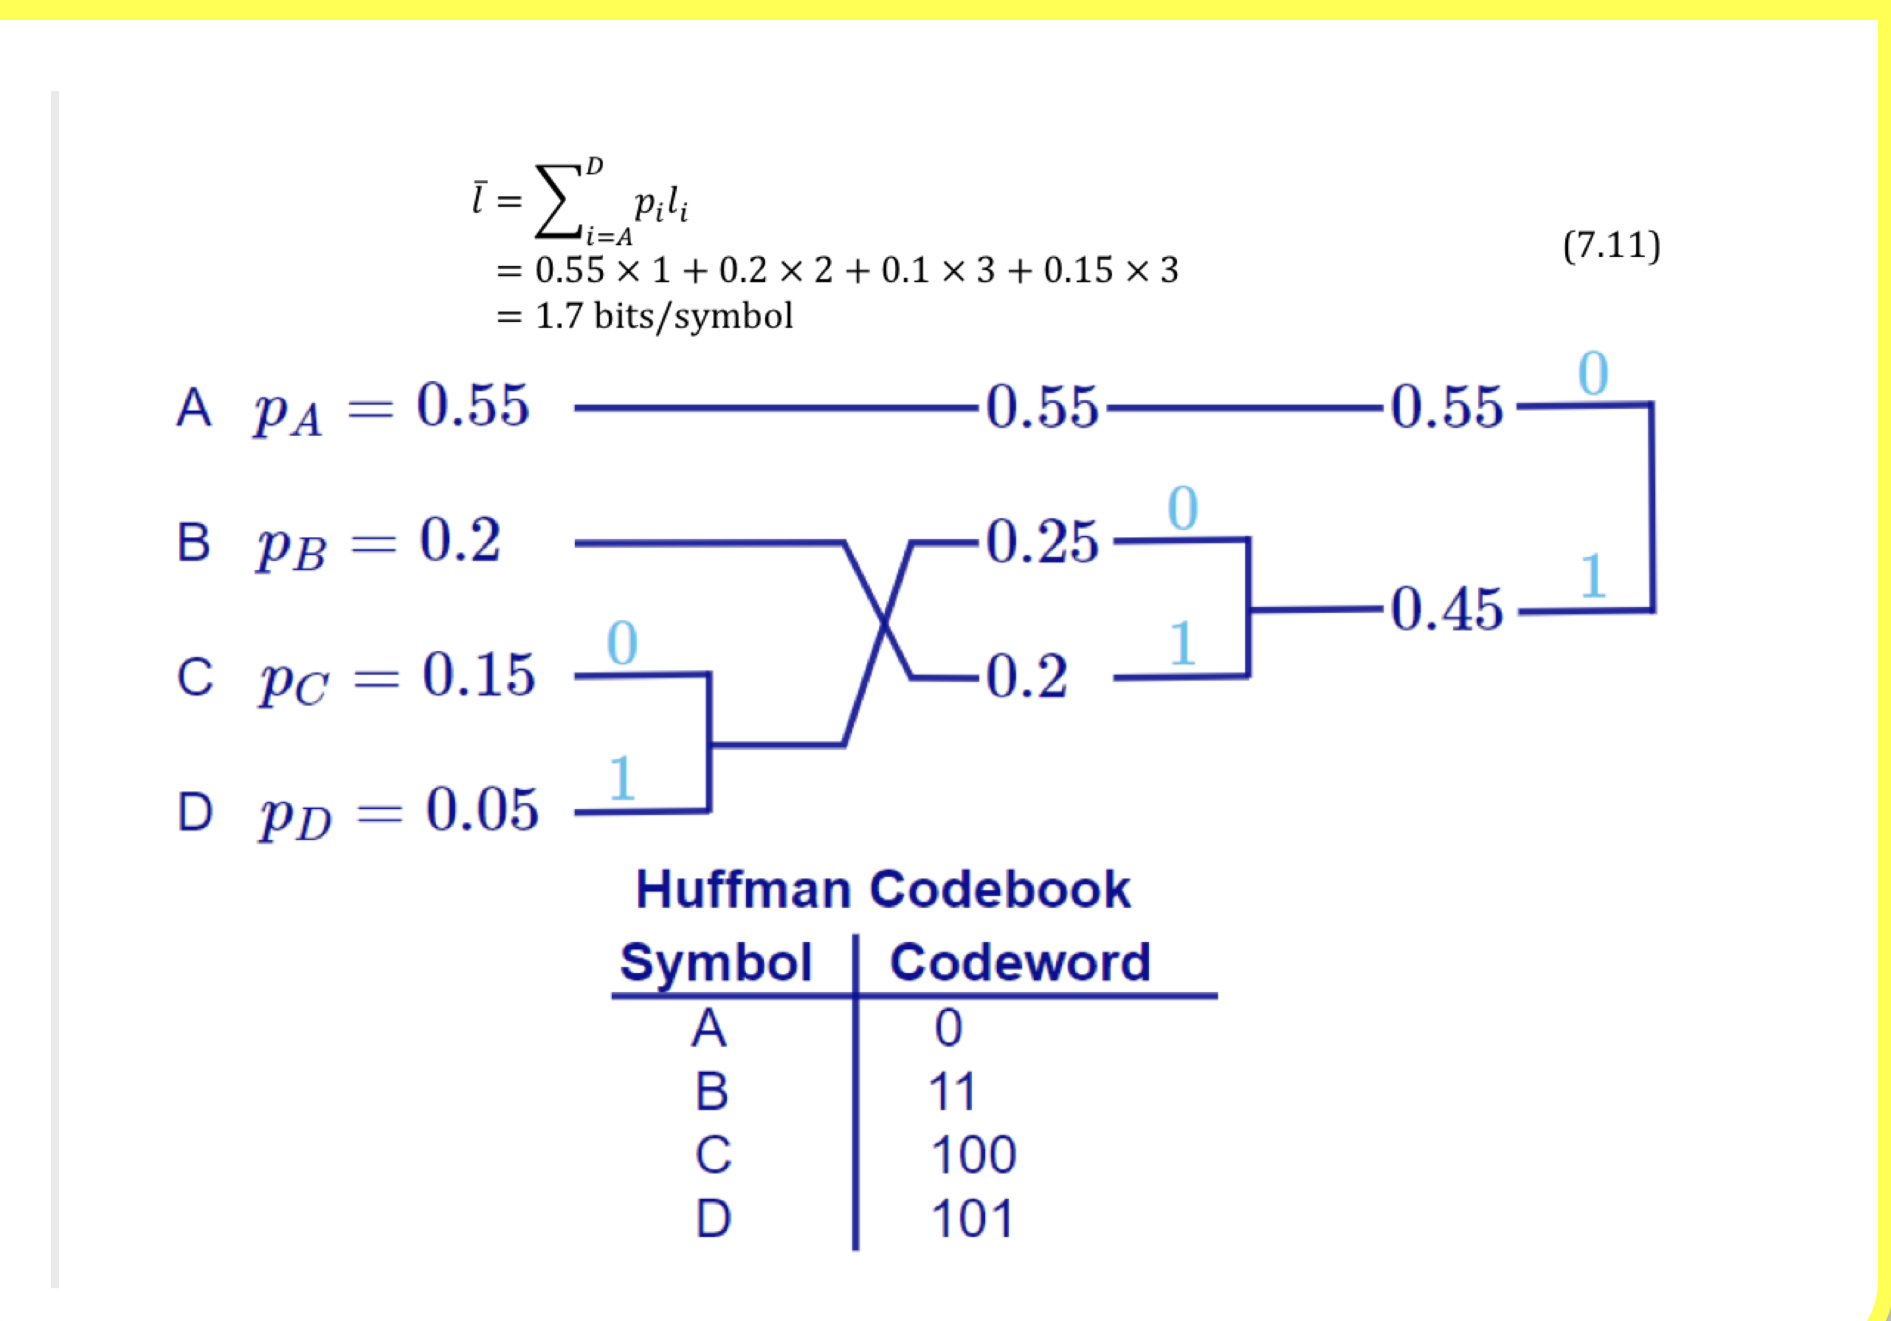
\includegraphics[width=\linewidth]{./huffman_code.jpeg}
\end{itemize}
%
\subsubsection*{DNS}
\begin{itemize}[noitemsep]
    \item \textbf{DNS Res.Record}  \verb|<Name,Class,TTL,Type,Value>|\\
    \item Type A: IPv4 32-bit
    \item Type AAAA: IPv6 128-bit
    \item Type NS:  hostname of the auth. NS, (hostname->hostn.)
    \item Type CNAME:  canonical hostname (hostname->hostn.)
    \item Type MX:  hostname of mail server (hostname->hostn.)
    \item Caveat: for the 3 above, require another A record for hostn.
    \item Recursive Query: DNS server queries lower level for u
    \item Iterative Query: DNS server returns queries, u go fetch other DNS servers
\end{itemize}

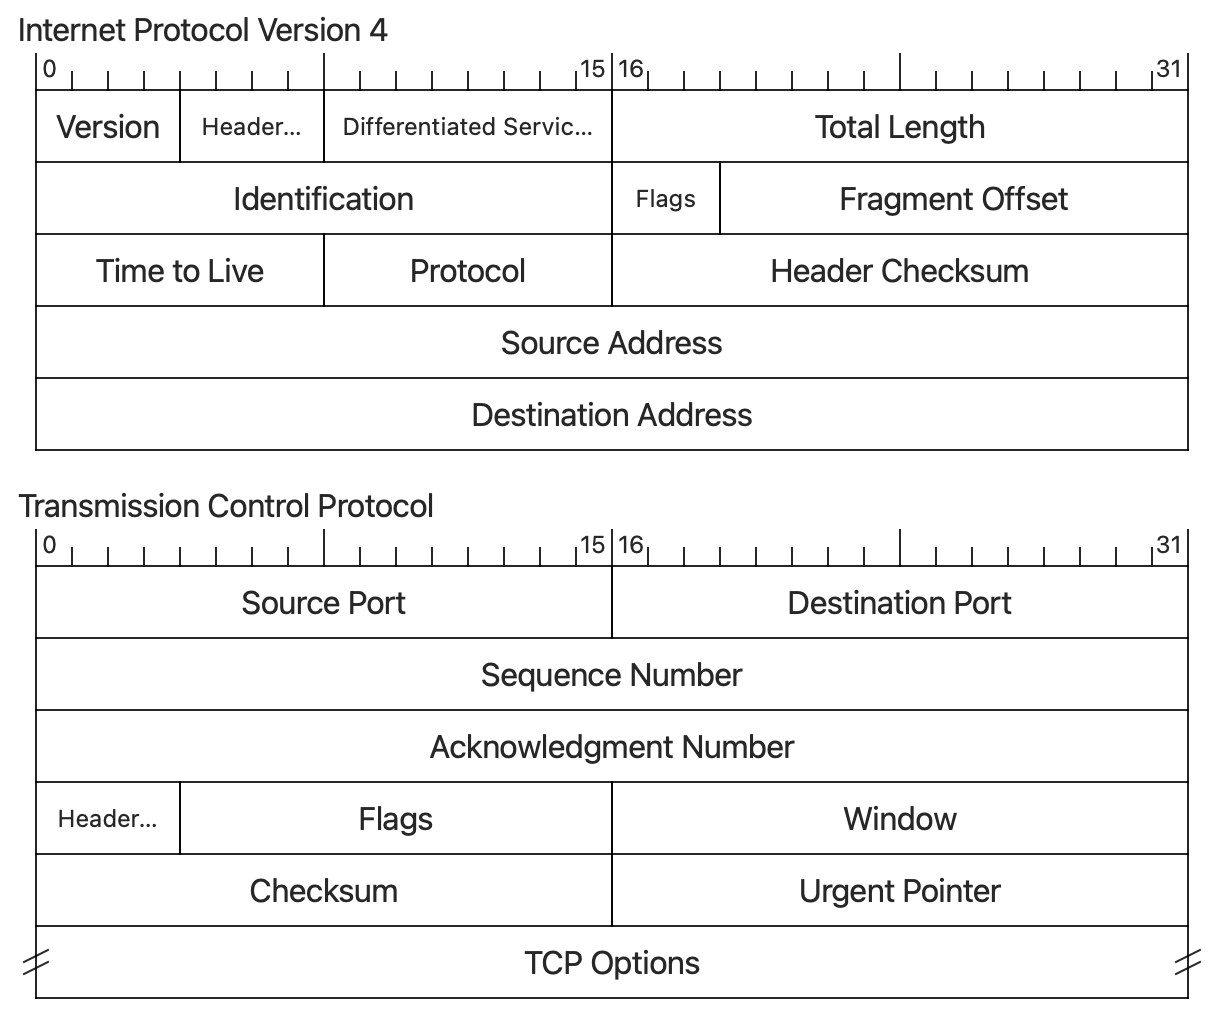
\includegraphics[width=\linewidth]{subfiles/Header_compact.png}

\problem{H1}

\problem{H2}
\begin{itemize}
    \item Two different implementations. 1) Star Topology w/ Hub. Hub bad, because hub is just a multi-port repeater.
    \item All cables from terminals go into different ports of hub, and hub amplifies and regens the signal, and transmits to ALL OTHER active ports.
    \item But Hub better than BUS, because easy deployment.

    \item 2) Star Topology w/ Switch. Switch good, because improved network efficiency.

\item Components of Switch: Port buffer: obvious Switching fabric: does not forward incoming signal to everyone, determination of destination of datagrams.

\item Addressing done by MAC addresses in incoming headers.

\item Scenario: Two frames incoming, each has different destination. Switching fabric can forward to two different ports. no collision occurs.
We call this: separate collision domains. (The destination ports are the collision domains).

\item Full Duplex efficiency: Given each temrinal has two ports (one input and output), then the terminal can send and receive at the same time. Very good basadao techinology yeahhhhh
\item why bus bad, bc broadcast domain lots of collisions and prob of collide inceases with temrinals. maintanece hard, need phsyicall attach cable.
\item star topology usin ghub ( bad), star topology using switch ( good)

\end{itemize}

\subsubsection*{Spanning Tree Algorithm}

\begin{enumerate}[noitemsep]
    \item \verb|root_node|: smallest ID
    \item \verb|root_port|: each non root bridge, elect port w/ lowest cost to root
    \item   \verb|designated_port|: for each line segment, choose port w/ lowest bridge ID to DP
    \item Step4: block all other ports
    \item Tiebreak: according to bridgeID then portID
\end{enumerate}

\problem{H3}
\subsubsection*{Cellular Networks}

\begin{itemize}[noitemsep]
    \item \textbf{N} freq. reuse fctr/ \# cells in clstr
    \item \textbf{$\alpha$}  pthlss exponent
    \item \textbf{$L$} \# of 1st odr intrfrng cells
    \item \textbf{SIR} $\frac{(3N)^{\alpha/2}}{L}$
\end{itemize}
\begin{itemize}[noitemsep]
    \item $T$: total spectrum alotted, 
    \item $B_c$: spec. requirement of one channel.
    \item $K$: \# of cells/cluster,
    \item $\text{\# of channels/cell}=(T/B_c)/K$
\end{itemize}
\subsubsection{wireless csma}
\tiny{\begin{itemize}
    \item hidden station: channel sens does not necessarily yield correct conc. whether to transm.
    \item prevent A, C hear each other, even tho A and C trans are interfering at B
    \item exposed station, sensing does not necessarily yield correct conc. whether to transm.
    \item D close to A, but not close to B, A can transm to B but not allowed.
    \item RTS/CTS: transmitter to send RTS first, indiciating time to transm.
    \item receiver reply with CTS, serves two purposes (instructs other stsations not to transm.) and (gives sender explit permission to send.)
    \item when wireless: hard to detect collisions at adapter.
    \item multipath fading: env changes drastically w/ time, superimposed atten and phases with direct signal.
    \item csma/ca: transm. after difs, and acks allowed after sifs to priotiize. 
    \item require link level ack.
\end{itemize}}


\subfile{./q1.tex}
\subfile{./q2.tex}
\subfile{./q3.tex}
\subfile{./q4.tex}
\subfile{./q5.tex}
\subfile{./q6.tex}
\subfile{./q7.tex}
\subfile{./q8.tex}
\subfile{./q9.tex}
\subfile{./q10.tex}
\subfile{./q11.tex}
\subfile{./q12.tex} % \vfill\null\columnbreak
\subfile{./q13.tex}
\subfile{./q14.tex}
\subfile{./q15.tex}
\subfile{./q16.tex}
\subfile{./q17.tex}
\subfile{./q18.tex}
\subfile{./q19.tex}
\subfile{./q20.tex}

\subsubsection*{factoids}
\begin{itemize}
    \item Cyclic prefix good. because makes it periodic signal
    \item Free space path gain, $\lambda$ wavelength. $P_r/P_t = (\lambda/(4\pi d))^2$

\item Antenna, equivalent gain (isotropic source) $G = I/I_{iso}$

\item Effective Isotropic Area $A_{eff}=(\lambda^2)/(4\pi)G$

\item Effective Isotropic Radiated Power $EIRP = PG$

\item Infinite bandwidth, $\lim_{\epsilon_{max}\to 0}(E_b/N_0)=\log_e2 = 0.693$ minimal SNR

\item Stop and Wait Delay minimal$T\geq 2t_p + t_i$. $t_p$ prop time, $t_i$ transmission of data frame. delay bandwidth product.

\item Dijsktra vs Bellman Ford, Count to Infinity issue. AB link die, B falsely learns from C it cna reach A. So cost \verb|BA = CB + AC(fake)|, and on next round C learns again, so adds another \verb|CB|, since it sensed AB cost updated (increased).
\item: bellman: convergence may have loop. dijkstra, $n^2$, may oscillate. bellman: error can propgate thru entire network.
\item CDMA: adv: multple users same time, low interference, wide band hard to jam. code secure, frequency diversity, good for frequency dependent impairments. wide bw means can transm. at low SNR.
\item CDMA disadv: require large bandwidth, complex system, near-far problem. when unintended transm. is closer than the intended transm.
\item video frame: I data, compressed jpeg images, P- interframe compress with relation to previous I/P frames, b frame; bidirectional - compressing using before and after IP frames. highst rate of comp.
\item gop size: distance bewteen 2 I frames. frame pattern, the pattern of P I, etc.

\end{itemize}
\end{multicols}
\end{document}

% Each subfile is individually exportable for easy Crowdmark handling.
% The purpose of this file is to make it so that all other files can use the import function on Overleaf. This is not a template. Rather assignment templates should import from this file. On cloning the assignment template, the cloned file will still reference this file, and any edits in the header files will take one refresh as opposed to 3-4.
